\documentclass[preview]{standalone}

\usepackage{amsmath}
\usepackage{amssymb}
\usepackage{stellar}
\usepackage{definitions}
\usepackage{bettelini}
\usepackage{tikz}

\begin{document}

\id{graph-complete-bipartite}
\genpage

\section{Complete graphs}

\begin{snippetdefinition}{complete-graph-definition}{Complete graph}
    Let \(n\in\integers^+\). The \emph{complete graph} \(K_n\) is the simple
    \graph with \(n\) vertices in which every pair of distinct vertices is
    joined by an edge.
    In particular,
    \[
        \cardinality{V(K_n)}=n,
        \qquad
        \cardinality{E(K_n)}=\binom{n}{2}=\frac{n(n-1)}{2}.
    \]
\end{snippetdefinition}

\begin{snippetexample}{small-complete-graphs-planar-example}{Small complete graphs}
    The graphs \(K_n\) are planar for \(n\leq 4\):
    \[
        \begin{tikzpicture}[scale=1]
            \begin{scope}
                \fill (0,0) circle (1.8pt);
                \node at (0,-0.45) {\(n=1\)};
            \end{scope}

            \begin{scope}[xshift=2.4cm]
                \coordinate (a) at (0,0);
                \coordinate (b) at (1,0);
                \draw (a)--(b);
                \fill (a) circle (1.8pt);
                \fill (b) circle (1.8pt);
                \node at (0.5,-0.45) {\(n=2\)};
            \end{scope}

            \begin{scope}[xshift=5cm]
                \coordinate (a) at (0,0);
                \coordinate (b) at (1,0);
                \coordinate (c) at (0.5,0.85);
                \draw (a)--(b)--(c)--cycle;
                \foreach \p in {a,b,c}{
                    \fill (\p) circle (1.8pt);
                }
                \node at (0.5,-0.45) {\(n=3\)};
            \end{scope}

            \begin{scope}[xshift=8cm]
                \coordinate (a) at (0,0);
                \coordinate (b) at (1,0);
                \coordinate (c) at (1,1);
                \coordinate (d) at (0,1);
                \draw (a)--(b)--(c)--(d)--cycle;
                \draw (d)--(b);
                \draw (a) .. controls +(-0.75,0.30) and +(-1.05,0.75) .. (c);
                \foreach \p in {a,b,c,d}{
                    \fill (\p) circle (1.8pt);
                }
                \node at (0.5,-0.45) {\(n=4\)};
            \end{scope}
        \end{tikzpicture}
    \]
\end{snippetexample}

\begin{snippetproposition}{complete-graph-k5-nonplanar}{The graph \(K_5\) is not planar}
    The complete graph \(K_5\) is not planar. Consequently, \(K_n\) is not
    planar for every \(n\geq 5\).
\end{snippetproposition}

\begin{snippetproof}{complete-graph-k5-nonplanar-proof}{complete-graph-k5-nonplanar}{The graph \(K_5\) is not planar}
    Suppose for contradiction that \(K_5\) is planar. Then
    \[
        v=5,
        \qquad
        e=\frac{5\cdot 4}{2}=10.
    \]
    By \snippetref[euler-formula-planar-graphs][Euler's formula],
    \[
        5-10+f=2,
    \]
    so \(f=7\).

    Since \(K_5\) is simple, every face is bounded by at least \(3\) edges.
    Summing the boundary lengths over all faces gives at least
    \[
        3f=21.
    \]
    On the other hand, every edge can bound at most two faces, so the same sum
    is at most
    \[
        2e=20.
    \]
    Hence \(21\leq 20\), a contradiction.

    Therefore \(K_5\) is not planar. If \(n\geq 5\), then \(K_n\) contains a
    subgraph isomorphic to \(K_5\). If \(K_n\) were planar, every subgraph would
    be planar, in particular \(K_5\), contradiction.
\end{snippetproof}

\section{Bipartite graphs}

\begin{snippetdefinition}{bipartite-graph-definition}{Bipartite graph}
    A \graph \(G\) is \emph{bipartite} if its vertex set can be written as a
    disjoint union
    \[
        V(G)=V_1\union V_2,
        \qquad
        V_1\intersection V_2=\emptyset,
    \]
    with \(V_1,V_2\neq\emptyset\), such that every edge joins a vertex of
    \(V_1\) to a vertex of \(V_2\).
    In particular, a bipartite graph has no loops and no edge joining two
    vertices in the same part.
\end{snippetdefinition}

\begin{snippetdefinition}{complete-bipartite-graph-definition}{Complete bipartite graph}
    Let \(m,n\in\integers^+\). The \emph{complete bipartite graph}
    \(K_{m,n}\) is the simple \graph whose vertex set is a disjoint union
    \[
        V_1\union V_2,
        \qquad
        \cardinality{V_1}=m,
        \qquad
        \cardinality{V_2}=n,
    \]
    and whose edges join every vertex of \(V_1\) to every vertex of \(V_2\).
    In particular,
    \[
        \cardinality{V(K_{m,n})}=m+n,
        \qquad
        \cardinality{E(K_{m,n})}=mn.
    \]
\end{snippetdefinition}

\begin{snippetexample}{complete-bipartite-k23-example}{The graph \(K_{2,3}\)}
    The graph \(K_{2,3}\) is planar:
    \[
        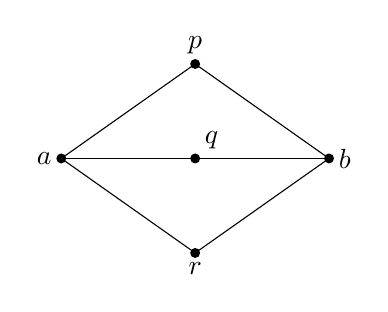
\begin{tikzpicture}[scale=1]
            \coordinate (a) at (-1.7,0);
            \coordinate (b) at (1.7,0);
            \coordinate (p) at (0,1.2);
            \coordinate (q) at (0,0);
            \coordinate (r) at (0,-1.2);

            \draw (a)--(p)--(b);
            \draw (a)--(q)--(b);
            \draw (a)--(r)--(b);

            \foreach \x in {a,b,p,q,r}{
                \fill (\x) circle (1.8pt);
            }

            \node[left] at (a) {\(a\)};
            \node[right] at (b) {\(b\)};
            \node[above] at (p) {\(p\)};
            \node[above right] at (q) {\(q\)};
            \node[below] at (r) {\(r\)};
        \end{tikzpicture}
    \]
    The two parts of the bipartition are
    \[
        V_1=\{a,b\},
        \qquad
        V_2=\{p,q,r\}.
    \]
\end{snippetexample}

\begin{snippetproposition}{complete-bipartite-k33-nonplanar}{The graph \(K_{3,3}\) is not planar}
    The complete bipartite graph \(K_{3,3}\) is not planar.
\end{snippetproposition}

\begin{snippetproof}{complete-bipartite-k33-nonplanar-proof}{complete-bipartite-k33-nonplanar}{The graph \(K_{3,3}\) is not planar}
    Suppose for contradiction that \(K_{3,3}\) is planar. Then
    \[
        v=6,
        \qquad
        e=9.
    \]
    By \snippetref[euler-formula-planar-graphs][Euler's formula],
    \[
        6-9+f=2,
    \]
    so \(f=5\).

    Every face must be bounded by at least \(4\) edges. Indeed, if a face were
    bounded by \(3\) edges, those three vertices would form a triangle. But a
    bipartite graph has no triangles.

    Therefore, summing the boundary lengths of all faces gives at least
    \[
        4f=20.
    \]
    On the other hand, every edge can bound at most two faces, so the same sum
    is at most
    \[
        2e=18.
    \]
    Hence \(20\leq 18\), a contradiction. Therefore \(K_{3,3}\) is not
    planar.
\end{snippetproof}

\begin{snippettheorem}{kuratowski-theorem}{Kuratowski's theorem}
    A finite \graph is non-planar \ifandonlyif it contains a subdivision of
    \(K_5\) or a subdivision of \(K_{3,3}\).

    Here, \emph{contains} means that the graph contains as a subgraph a graph
    obtained from \(K_5\) or \(K_{3,3}\) by subdividing some edges, that is, by
    replacing those edges with paths whose internal vertices are new.
\end{snippettheorem}

\end{document}
